\documentclass[12pt,a4paper]{article}

% --------------------------------------------------
% Pacotes
% --------------------------------------------------
\usepackage[T1]{fontenc}
\usepackage[utf8]{inputenc}
\usepackage[main=brazil]{babel}

\usepackage[
    a4paper,
    margin=2.5cm,
    top=3.2cm,
    headheight=70pt,
    headsep=18pt
]{geometry}
\usepackage{graphicx}

\usepackage{amsmath,amssymb}
\usepackage{caption}
\usepackage{setspace}
\usepackage{titlesec}
\usepackage{indentfirst}
\usepackage{float}
\usepackage{newtxtext,newtxmath}
\usepackage[hidelinks]{hyperref}
\usepackage{fancyhdr}

% --------------------------------------------------
% Cabeçalho
% --------------------------------------------------
\pagestyle{fancy}
\fancyhf{}
\fancyhead[R]{
\includegraphics[height=1.8cm]{base_images/logo-puc.png}}
\renewcommand{\headrulewidth}{0pt}

% --------------------------------------------------
% Ajustes visuais
% --------------------------------------------------
\setlength{\parindent}{1.25cm}
\setlength{\parskip}{0pt}
\onehalfspacing

\captionsetup{
    font=small,
    labelfont=normalfont,
    justification=centering
}

\titleformat{\subsection}
  {\normalfont\bfseries\large}
  {\thesubsection}
  {0.6em}
  {}

% --------------------------------------------------
% Comandos úteis
% --------------------------------------------------
\newcommand{\question}[1]{
    \vspace{0.8em}
    \noindent\textit{#1}
    \vspace{0.4em}
}

\newcommand{\answer}{
    \par
}

% Placeholder de figura ainda não gerada (compila sem a imagem).
% Quando o print estiver pronto, comente a \placeholderfig e ative o \includegraphics.
\newcommand{\placeholderfig}[1]{%
    \fbox{\parbox[c][4cm][c]{0.98\linewidth}{\centering\itshape [Figura pendente: #1]}}%
}

% --------------------------------------------------
% Documento
% --------------------------------------------------
\begin{document}

% Título
\begin{center}
    {\LARGE \textbf{ENG4448 - Laboratório de Computação Digital}}\\[0.3cm]
    {\Large Relatório do Laboratório 09}\\[0.2cm]
    % TODO: ajustar a data do laboratório
    06/10/2026 - Rio de Janeiro
\end{center}

\vspace{0.8cm}

% Informações da dupla
\noindent \textbf{Turma 3VA - Dupla:}\\
Pedro Coelho Carneiro da Cunha - 2310837\\
Pedro Carneiro Nogueira - 2310540

\vspace{0.5cm}
\hrule
\vspace{0.8cm}

\setcounter{section}{1}
\setcounter{subsection}{0}

\section{Roteiro}

% ==============================================================
\subsection{Exercício 1 – Comunicação SPI}
% ==============================================================

\question{Crie um novo projeto no Xilinx ISE Project Navigator e um módulo VHDL responsável
por controlar o ADC via SPI e interpretar os dados recebidos. Configure o pré-amplificador,
o ADC e desabilite os demais dispositivos SPI do kit.}

\answer
O circuito de captura analógica do \textit{Spartan-3E Starter Kit} é formado por dois
componentes em cascata no mesmo barramento SPI (UG230, Capítulo~10): o pré-amplificador
programável \texttt{LTC6912-1} e o conversor A/D \texttt{LTC1407A-1}. A implementação foi
organizada em dois arquivos VHDL: o módulo de controle (\texttt{adc\_ctrl.vhd}), que
concentra toda a lógica SPI e o mapeamento para os LEDs, e o módulo de topo
(\texttt{top.vhd}), de arquitetura estrutural, que instancia o controlador e desabilita os
demais dispositivos do barramento.

\subsubsection{Geração do \textit{clock} SPI}

O \texttt{SPI\_SCK} é derivado do \textit{clock} de 50\,MHz da placa por um divisor
(\textit{generic} \texttt{DIV\_FACTOR = 8}): o sinal é invertido a cada 8 ciclos de
\texttt{CLK50}, resultando em um período de 320\,ns ($\approx$3{,}125\,MHz), com folga
confortável em relação às taxas máximas suportadas tanto pelo \texttt{LTC6912-1} quanto pelo
\texttt{LTC1407A-1}. O mesmo processo gera dois pulsos de largura unitária, \texttt{sck\_rise}
e \texttt{sck\_fall}, que sinalizam as bordas de subida e descida do \texttt{SPI\_SCK} e
sincronizam a máquina de estados. Adota-se a convenção \texttt{CPOL = 0}, \texttt{CPHA = 0}:
o \texttt{SPI\_MOSI} é alterado na borda de \textbf{descida} (o amplificador o amostra na
subida) e o \texttt{SPI\_MISO} é amostrado na borda de \textbf{subida} (o ADC o apresenta na
descida).

\subsubsection{Máquina de estados}

O núcleo do módulo é uma FSM de seis estados (Tabela~\ref{tab:fsm}) que executa, em cada
volta, a configuração do amplificador seguida de uma leitura completa do ADC.

\begin{table}[H]
\centering
\begin{tabular}{ll}
\hline
\textbf{Estado} & \textbf{Função} \\
\hline
\texttt{AMP\_CS\_LOW} & Abaixa \texttt{AMP\_CS} (com SCK baixo) e apresenta o 1º bit da palavra de ganho \\
\texttt{AMP\_SHIFT}   & Desloca os 8 bits da palavra de ganho em \texttt{SPI\_MOSI} \\
\texttt{AMP\_LATCH}   & Levanta \texttt{AMP\_CS}, aplicando o ganho ao amplificador \\
\texttt{ADC\_PREP}    & Asserta \texttt{AD\_CONV} (com SCK baixo) para iniciar a conversão \\
\texttt{ADC\_READ}    & Lê 34 ciclos de \texttt{SPI\_MISO} para o registrador de deslocamento \\
\texttt{ADC\_LATCH}   & Extrai o canal A, calcula o nível e atualiza os LEDs \\
\hline
\end{tabular}
\caption{Estados da FSM de \texttt{adc\_ctrl.vhd}.}
\label{tab:fsm}
\end{table}

\paragraph{Configuração do amplificador.}
A palavra de ganho do \texttt{LTC6912-1} tem 8 bits no formato
\texttt{[B3 B2 B1 B0 A3 A2 A1 A0]}, enviados com o bit mais significativo primeiro. Para
ganho $-1$, o código de cada canal é \texttt{0001} (Tabela~10-2 do UG230), resultando na
constante \texttt{AMP\_GAIN\_WORD = "00010001"} (0x11). Os 8 bits são deslocados em
\texttt{SPI\_MOSI} a cada descida de \texttt{SPI\_SCK}; ao final, \texttt{AMP\_CS} retorna a
`1', latcheando o ganho no amplificador.

\paragraph{Leitura do ADC.}
Com \texttt{AD\_CONV} assertado, o \texttt{LTC1407A-1} inicia a conversão e transmite uma
sequência de 34 ciclos (UG230, Fig.~10-6). O quadro serial tem o formato:
\begin{center}
    2 ciclos em alta impedância \;$|$\; canal A (14 bits) \;$|$\; 2 ciclos \;$|$\;
    canal B (14 bits) \;$|$\; 2 ciclos.
\end{center}
Os bits são amostrados nas subidas de \texttt{SPI\_SCK} e acumulados no registrador de
deslocamento \texttt{adc\_shift}; após os 34 ciclos, os 14 bits do canal A
(\texttt{VINA}) são extraídos (\texttt{adc\_shift(30 downto 17)}). O sinal \texttt{AD\_CONV}
é rebaixado logo após a primeira borda de subida.

\subsubsection{Interpretação do valor e acionamento dos LEDs}

O canal A é lido em complemento de 2 (\texttt{signed}, faixa $-8192$ a $8191$). Como o
amplificador tem ganho $-1$, a tensão de entrada cresce à medida que o código digital fica
mais negativo. Para obter um nível crescente com a tensão, aplica-se
$\texttt{lvl} = 8191 - \texttt{ch0}$ (faixa 0 a 16383) e mapeia-se para o número de LEDs
acesos por $n = \lfloor \texttt{lvl} \times 9 / 16384 \rfloor$ (0 a 8). Os LEDs são acesos
em barra: à medida que a tensão aumenta, mais LEDs acendem sequencialmente, de nenhum LED
(faixa mínima) até os oito LEDs (faixa máxima). A Tabela~\ref{tab:led_scale} apresenta a
escala de ativação obtida (script \texttt{led\_scale.py}), dividindo proporcionalmente a
faixa do ADC.

\begin{table}[H]
\centering
\begin{tabular}{ccc}
\hline
\textbf{LEDs acesos} & \textbf{D[13:0] (decimal)} & \textbf{$V_{IN}$ (V)} \\
\hline
0 & \phantom{-}6371 \dots \phantom{-}8191 & 0{,}400 \dots 0{,}678 \\
1 & \phantom{-}4551 \dots \phantom{-}6370 & 0{,}678 \dots 0{,}956 \\
2 & \phantom{-}2730 \dots \phantom{-}4550 & 0{,}956 \dots 1{,}233 \\
3 & \phantom{-}\phantom{0}910 \dots \phantom{-}2729 & 1{,}234 \dots 1{,}511 \\
4 & $-911$ \dots \phantom{-}\phantom{0}909 & 1{,}511 \dots 1{,}789 \\
5 & $-2731$ \dots $-912$ & 1{,}789 \dots 2{,}067 \\
6 & $-4552$ \dots $-2732$ & 2{,}067 \dots 2{,}345 \\
7 & $-6372$ \dots $-4553$ & 2{,}345 \dots 2{,}622 \\
8 & $-8192$ \dots $-6373$ & 2{,}622 \dots 2{,}900 \\
\hline
\end{tabular}
\caption{Escala de ativação dos LEDs em função do código do ADC e da tensão de entrada
         (ganho $-1$, faixa 0{,}4\,V a 2{,}9\,V).}
\label{tab:led_scale}
\end{table}

\subsubsection{Módulo de Topo (\texttt{top.vhd})}

O módulo de topo instancia \texttt{adc\_ctrl} e, para evitar contenção no barramento SPI
compartilhado, mantém os demais dispositivos permanentemente desabilitados
(Tabela~10-4 do UG230): \texttt{SPI\_SS\_B = '1'} (\textit{StrataFlash}),
\texttt{DAC\_CS = '1'} (DAC), \texttt{SF\_CE0 = '1'} (\textit{StrataFlash} CE) e
\texttt{FPGA\_INIT\_B = '0'} (PROM de plataforma).

% ==============================================================
\subsection{Exercício 2 – Simulação}
% ==============================================================

\question{Após concluir a implementação, crie um testbench para validar o protocolo de
comunicação. Verifique a ordem de envio dos bits. Lembre-se de alterar \texttt{clk\_period}
para 20\,ns.}

\answer
Foram desenvolvidos dois \textit{testbenches}, ambos com \texttt{clk\_period = 20\,ns}
(50\,MHz): \texttt{adc\_ctrl\_tb.vhd}, que valida o controlador isoladamente, e
\texttt{top\_tb.vhd}, que exercita o módulo de topo integrado.

\subsubsection{\textit{Testbench} do Controlador (\texttt{adc\_ctrl\_tb.vhd})}

O \textit{testbench} inclui um modelo comportamental do ADC: o processo \texttt{miso\_proc}
apresenta o bit do ciclo~1 na subida de \texttt{AD\_CONV} e avança um bit a cada descida de
\texttt{SPI\_SCK}, reproduzindo o quadro de 34 ciclos. O vetor de teste \texttt{MISO\_VEC}
foi montado com o canal A igual a \texttt{"10000000000000"} ($-8192$ em complemento de 2),
o que corresponde à tensão máxima e, portanto, aos oito LEDs acesos. Após 60\,$\mu$s
(tempo suficiente para a configuração do amplificador e algumas leituras), o estímulo
verifica \texttt{LEDS = "11111111"} — validando simultaneamente a ordem de envio dos bits e
o mapeamento para os LEDs. A Figura~\ref{fig:sim_amp} mostra a configuração do amplificador
e a Figura~\ref{fig:sim_adc}, a leitura do ADC.

\begin{figure}[H]
    \centering
    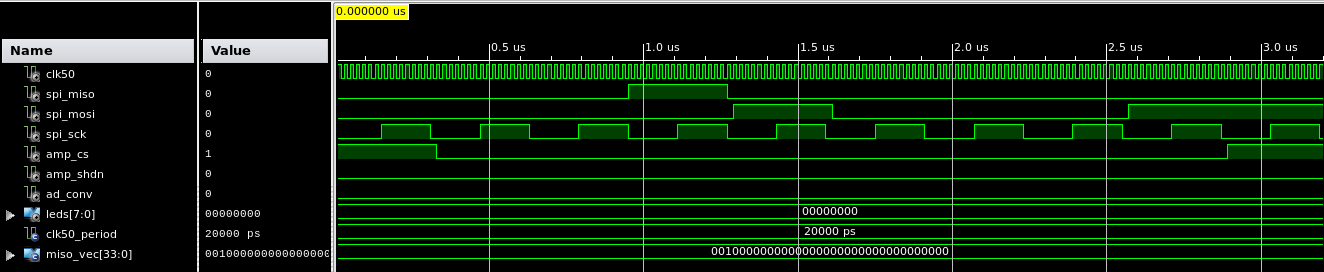
\includegraphics[width=\linewidth]{images/sim_amp.png}
    \caption{Forma de onda da configuração do pré-amplificador \texttt{LTC6912-1}:
             deslocamento da palavra de ganho \texttt{"00010001"} em \texttt{SPI\_MOSI}.}
    \label{fig:sim_amp}
\end{figure}

\begin{figure}[H]
    \centering
    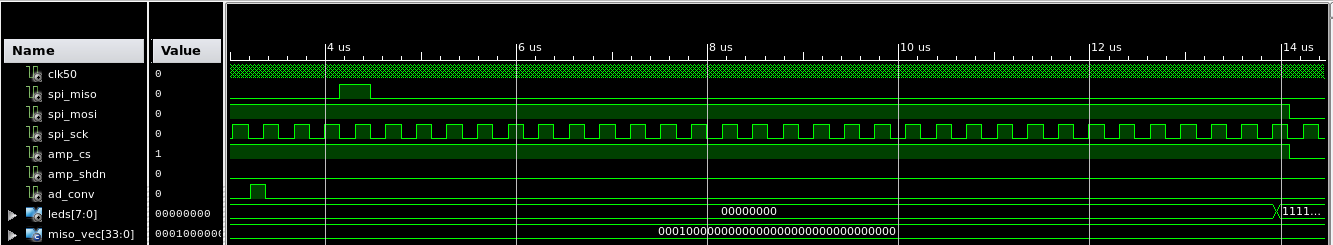
\includegraphics[width=\linewidth]{images/sim_adc.png}
    \caption{Forma de onda da leitura do ADC \texttt{LTC1407A-1}: \texttt{AD\_CONV} e os
             34 ciclos de \texttt{SPI\_SCK} amostrando \texttt{SPI\_MISO}.}
    \label{fig:sim_adc}
\end{figure}

\begin{figure}[H]
    \centering
    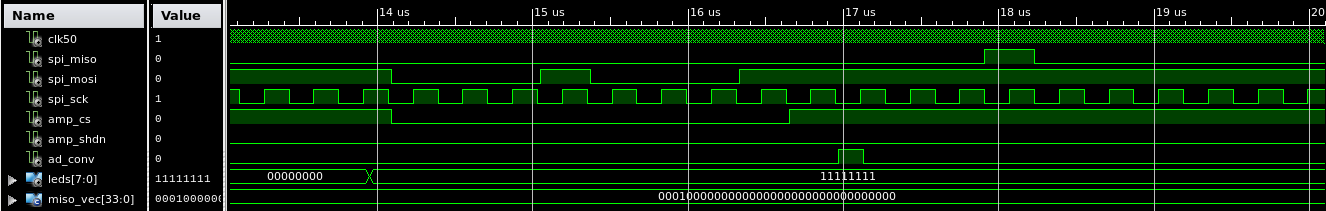
\includegraphics[width=\linewidth]{images/sim_leds.png}
    \caption{Resultado da simulação: \texttt{LEDS = "11111111"} (oito LEDs acesos) para o
             canal A no valor de fundo de escala.}
    \label{fig:sim_leds}
\end{figure}

\subsubsection{\textit{Testbench} do Módulo de Topo (\texttt{top\_tb.vhd})}

O \textit{testbench} de nível superior instancia \texttt{top} com todos os pinos, permitindo
confirmar que os sinais dos dispositivos desabilitados (\texttt{SPI\_SS\_B},
\texttt{DAC\_CS}, \texttt{SF\_CE0}, \texttt{FPGA\_INIT\_B}) assumem os valores corretos e que
a integração reproduz o comportamento observado no \textit{testbench} do controlador.

% ==============================================================
\subsection{Exercício 3 – Implementação e Teste na Placa}
% ==============================================================

\question{Faça a síntese, implementação e geração do arquivo \texttt{.bit}. Programe a placa
e verifique os LEDs acendendo de forma progressiva conforme a tensão na entrada do ADC
aumenta.}

\answer
O projeto foi sintetizado e implementado no Xilinx ISE Project Navigator para a FPGA
Spartan-3E (XC3S500E) do \textit{Spartan-3E Starter Kit}. O arquivo de restrições
\texttt{top.ucf} define as atribuições de pinos resumidas na Tabela~\ref{tab:pinos},
seguindo as figuras do Capítulo~10 do UG230.

\begin{table}[H]
\centering
\begin{tabular}{lll}
\hline
\textbf{Sinal} & \textbf{Pino} & \textbf{Função} \\
\hline
\texttt{CLK}        & C9  & \textit{clock} de 50\,MHz \\
\texttt{SPI\_SCK}   & U16 & \textit{clock} serial SPI \\
\texttt{SPI\_MOSI}  & T4  & dado serial para o amplificador \\
\texttt{SPI\_MISO}  & N10 & dado serial vindo do ADC \\
\texttt{AD\_CONV}   & P11 & início da conversão do ADC \\
\texttt{AMP\_CS}    & N7  & \textit{chip-select} do amplificador \\
\texttt{AMP\_SHDN}  & P7  & \textit{shutdown} do amplificador \\
\texttt{LEDS[7:0]}  & \multicolumn{2}{l}{F12, E12, E11, F11, C11, D11, E9, F9} \\
\texttt{SPI\_SS\_B} & U3  & \textit{StrataFlash} (desabilitado) \\
\texttt{DAC\_CS}    & N8  & DAC (desabilitado) \\
\texttt{SF\_CE0}    & D16 & \textit{StrataFlash} CE (desabilitado) \\
\texttt{FPGA\_INIT\_B} & T3 & PROM de plataforma (desabilitado) \\
\hline
\end{tabular}
\caption{Atribuição de pinos definida em \texttt{top.ucf}.}
\label{tab:pinos}
\end{table}

Após a geração do arquivo \texttt{.bit} e a programação da placa, o comportamento foi
validado girando o potenciômetro conectado à entrada do ADC: os LEDs discretos acendem de
forma progressiva (em barra) à medida que a tensão de entrada aumenta, de nenhum LED até os
oito LEDs acesos, conforme a escala da Tabela~\ref{tab:led_scale}.

O funcionamento completo na placa pode ser verificado no vídeo disponível em:
\begin{center}
    % TODO: inserir o link do vídeo
    \url{https://youtu.be/XXXXXXXXXXX}
\end{center}

\end{document}
